%% Document started, Sat Jul  3 19:30:52 CEST 2004, my 37th birthday,
%% while being stuck for 24 hours at Philadelphia airport, on my way 
%% back from the joint TIES/Accuracy 2004 symposium in Portland, ME.
%% Continued, Oct 28, during the Apmosphere mid-term review. Oh, shame.

% \VignetteIndexEntry{ The meuse data set: a tutorial for the gstat R package }

\documentclass[a4paper]{article}
\usepackage{hyperref}

\newcommand{\code}[1]{{\tt #1}}



\title{The meuse data set: a tutorial\\
for the {\tt gstat} R package }
\author{Edzer J.\ Pebesma}
\date{\today}

\usepackage{/usr/share/R/share/texmf/Sweave}
\begin{document}
\maketitle

\section{Introduction}
The \code{meuse} data set is a data set comprising of four heavy metals
measured in the top soil in a flood plain along the river Meuse. The
governing process seems that polluted sediment is carried by the river,
and mostly deposited close to the river bank. This document shows a
geostatistical analysis of this data set.

This tutorial introduced the functionality of the R package \code{gstat},
used in conjunction with package \code{sp}. Package \code{gstat} provides
a wide range of univariable and multivariable geostatistical modelling,
prediction and simulation functions, where package \code{sp} provides
general purpose classes and methods for defining, importing/exporting
and visualizing spatial data.

\section{R geostatistics packages}
Package \code{gstat} (Pebesma, 2004) is an R package that provides basic
functionality for univariable and multivariable geostatistical analysis,
including 
\begin{itemize}
\item variogram modelling, residual variogram modelling, and cross variogram
modelling using fitting of parametric models to sample variograms
\item geometric anisotropy specfied for each partial variogram model
\item restricted maximum likelihood fitting of partial sills 
\item variogram and cross variogram maps
\item simple, ordinary, universal and external drift (co)kriging
\item (sequential) Gaussian (co)simulation equivalents for each of
the kriging varieties
\item indicator (co)kriging and sequential indicator (co)simulation
\item kriging in a local or global neighbourhood 
\item block (co)kriging or simulation for each of the varieties, for
rectangular or irregular blocks
\end{itemize}
Other geostatistical packages for R usually lack part of these options
(e.g. block kriging, local kriging, or cokriging) but provide others:
e.g. package \code{geoR} and \code{geoRglm} (by Paulo Ribeiro and Ole
Christensen) provide the model-based geostatistics framework described
in Diggle et al. (1998), package \code{fields} (Doug Nychka and others)
provides thin plate spline interpolation, covariance functions for
spherical coordinates (unprojected data), and routines for network
design optimization.

\section{Spatial data frames}
Package \code{gstat} assumes that data are projected, i.e. they should
not be provided as lattitude/longitude. As an example, we will look
at the meuse data set, which is a regular data frame that comes with
package \code{gstat}:

\begin{Schunk}
\begin{Sinput}
> library(gstat)
\end{Sinput}
\begin{Soutput}
Loading required package: sp
\end{Soutput}
\begin{Sinput}
> data(meuse)
> class(meuse)
\end{Sinput}
\begin{Soutput}
[1] "data.frame"
\end{Soutput}
\begin{Sinput}
> names(meuse)
\end{Sinput}
\begin{Soutput}
 [1] "x"       "y"       "cadmium" "copper"  "lead"    "zinc"    "elev"   
 [8] "dist"    "om"      "ffreq"   "soil"    "lime"    "landuse" "dist.m" 
\end{Soutput}
\begin{Sinput}
> coordinates(meuse) = ~x + y
> class(meuse)
\end{Sinput}
\begin{Soutput}
[1] "SpatialPointsDataFrame"
attr(,"package")
[1] "sp"
\end{Soutput}
\begin{Sinput}
> summary(meuse)
\end{Sinput}
\begin{Soutput}
Object of class SpatialPointsDataFrame
Coordinates:
     min    max
x 178605 181390
y 329714 333611
Is projected: NA 
proj4string : [NA]
Number of points: 155
Data attributes:
    cadmium           copper            lead            zinc       
 Min.   : 0.200   Min.   : 14.00   Min.   : 37.0   Min.   : 113.0  
 1st Qu.: 0.800   1st Qu.: 23.00   1st Qu.: 72.5   1st Qu.: 198.0  
 Median : 2.100   Median : 31.00   Median :123.0   Median : 326.0  
 Mean   : 3.246   Mean   : 40.32   Mean   :153.4   Mean   : 469.7  
 3rd Qu.: 3.850   3rd Qu.: 49.50   3rd Qu.:207.0   3rd Qu.: 674.5  
 Max.   :18.100   Max.   :128.00   Max.   :654.0   Max.   :1839.0  
                                                                   
      elev             dist               om         ffreq  soil   lime   
 Min.   : 5.180   Min.   :0.00000   Min.   : 1.000   1:84   1:97   0:111  
 1st Qu.: 7.546   1st Qu.:0.07569   1st Qu.: 5.300   2:48   2:46   1: 44  
 Median : 8.180   Median :0.21184   Median : 6.900   3:23   3:12          
 Mean   : 8.165   Mean   :0.24002   Mean   : 7.478                        
 3rd Qu.: 8.955   3rd Qu.:0.36407   3rd Qu.: 9.000                        
 Max.   :10.520   Max.   :0.88039   Max.   :17.000                        
                                    NA's   : 2.000                        
    landuse       dist.m      
 W      :50   Min.   :  10.0  
 Ah     :39   1st Qu.:  80.0  
 Am     :22   Median : 270.0  
 Fw     :10   Mean   : 290.3  
 Ab     : 8   3rd Qu.: 450.0  
 (Other):25   Max.   :1000.0  
 NA's   : 1                   
\end{Soutput}
\begin{Sinput}
> coordinates(meuse)[1:5, ]
\end{Sinput}
\begin{Soutput}
          x      y
[1,] 181072 333611
[2,] 181025 333558
[3,] 181165 333537
[4,] 181298 333484
[5,] 181307 333330
\end{Soutput}
\begin{Sinput}
> bubble(meuse, "zinc", col = c("#00ff0088", "#00ff0088"), main = "zinc concentrations (ppm)")
\end{Sinput}
\end{Schunk}

% the following is needed because lattice plots (bubble wraps xyplot) do not
% show without an explicit print; in order not to confuse users, we hide this:
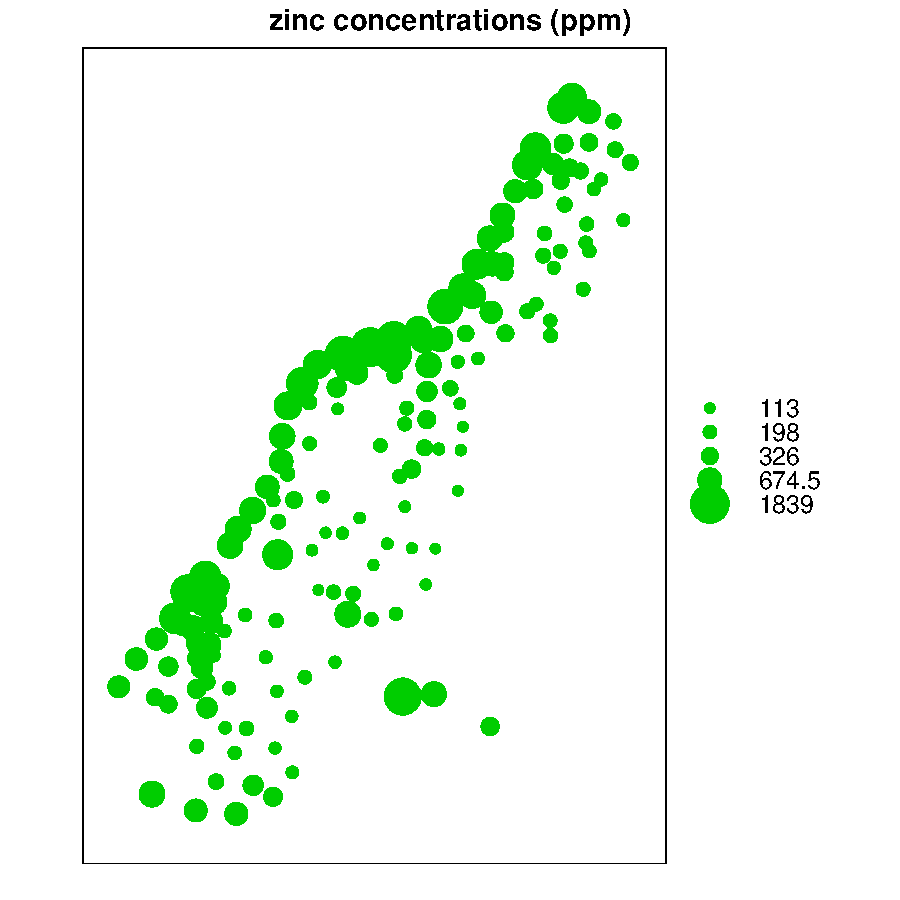
\includegraphics{gstat-002}

and note the following: 
\begin{enumerate}
\item the function \code{coordinates}, when assigned (i.e. on
the left-hand side of an \verb|=| or \verb|<-| sign), promotes the
\code{data.frame} meuse into a \code{SpatialPointsDataFrame}, which knows about
its spatial coordinates; coordinates may be specified by a formula,
a character vector, or a numeric matrix or data frame with the actual
coordinates
\item the function \code{coordinates}, when not assigned, {\em retrieves}
the spatial coordinates from a \code{SpatialPointsDataFrame}.
\item the two plotting functions used, \code{plot} and \code{bubble}
assume that the $x$- and $y$-axis are the spatial coordinates, and
choose the aspect ratio of the axes such that one unit in $x$
equals one unit in $y$ (i.e., data are map data, projected).
\end{enumerate}

\section{Spatial data on a regular grid}

\begin{Schunk}
\begin{Sinput}
> data(meuse.grid)
> summary(meuse.grid)
\end{Sinput}
\begin{Soutput}
       x                y              part.a           part.b      
 Min.   :178460   Min.   :329620   Min.   :0.0000   Min.   :0.0000  
 1st Qu.:179420   1st Qu.:330460   1st Qu.:0.0000   1st Qu.:0.0000  
 Median :179980   Median :331220   Median :0.0000   Median :1.0000  
 Mean   :179985   Mean   :331348   Mean   :0.3986   Mean   :0.6014  
 3rd Qu.:180580   3rd Qu.:332140   3rd Qu.:1.0000   3rd Qu.:1.0000  
 Max.   :181540   Max.   :333740   Max.   :1.0000   Max.   :1.0000  
      dist             soil       ffreq   
 Min.   :0.0000   Min.   :1.000   1: 779  
 1st Qu.:0.1193   1st Qu.:1.000   2:1335  
 Median :0.2715   Median :1.000   3: 989  
 Mean   :0.2971   Mean   :1.578           
 3rd Qu.:0.4402   3rd Qu.:2.000           
 Max.   :0.9926   Max.   :3.000           
\end{Soutput}
\begin{Sinput}
> class(meuse.grid)
\end{Sinput}
\begin{Soutput}
[1] "data.frame"
\end{Soutput}
\begin{Sinput}
> coordinates(meuse.grid) = ~x + y
> class(meuse.grid)
\end{Sinput}
\begin{Soutput}
[1] "SpatialPointsDataFrame"
attr(,"package")
[1] "sp"
\end{Soutput}
\begin{Sinput}
> gridded(meuse.grid) = TRUE
> class(meuse.grid)
\end{Sinput}
\begin{Soutput}
[1] "SpatialPixelsDataFrame"
attr(,"package")
[1] "sp"
\end{Soutput}
\begin{Sinput}
> image(meuse.grid["dist"])
> title("distance to river (red = 0)")
> zinc.idw = krige(zinc ~ 1, meuse, meuse.grid)
\end{Sinput}
\begin{Soutput}
[inverse distance weighted interpolation]
\end{Soutput}
\begin{Sinput}
> class(zinc.idw)
\end{Sinput}
\begin{Soutput}
[1] "SpatialPixelsDataFrame"
attr(,"package")
[1] "sp"
\end{Soutput}
\begin{Sinput}
> spplot(zinc.idw["var1.pred"], main = "zinc inverse distance weighted interpolations")
\end{Sinput}
\end{Schunk}
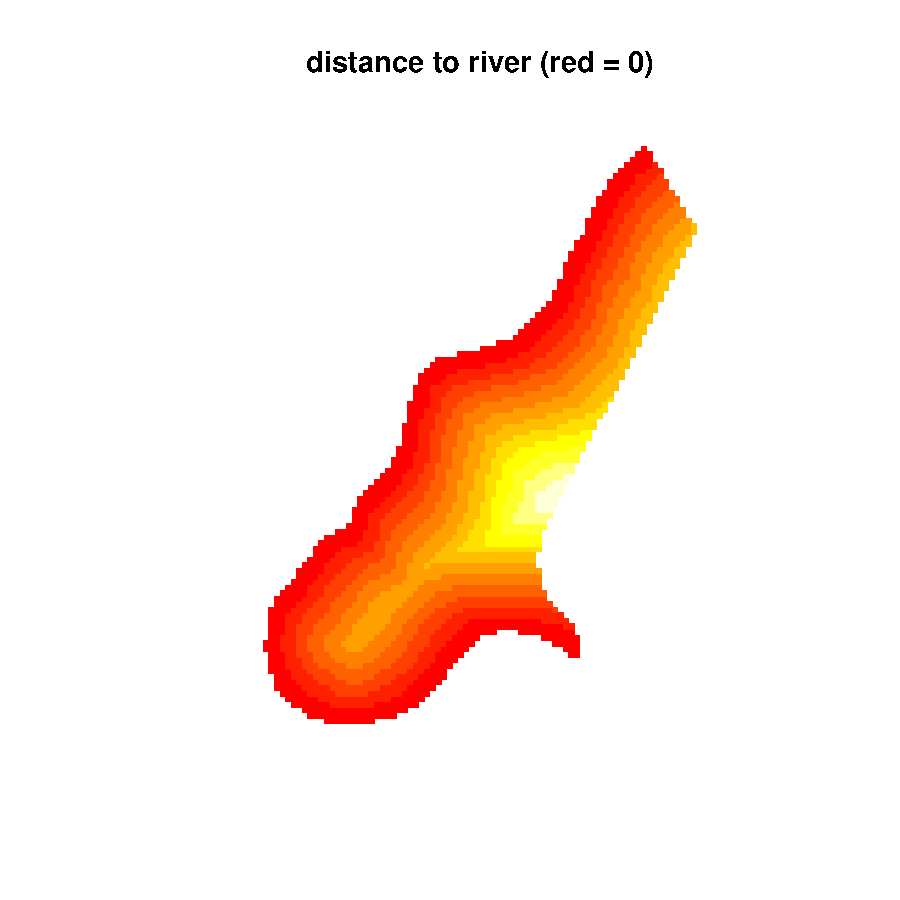
\includegraphics{gstat-003}

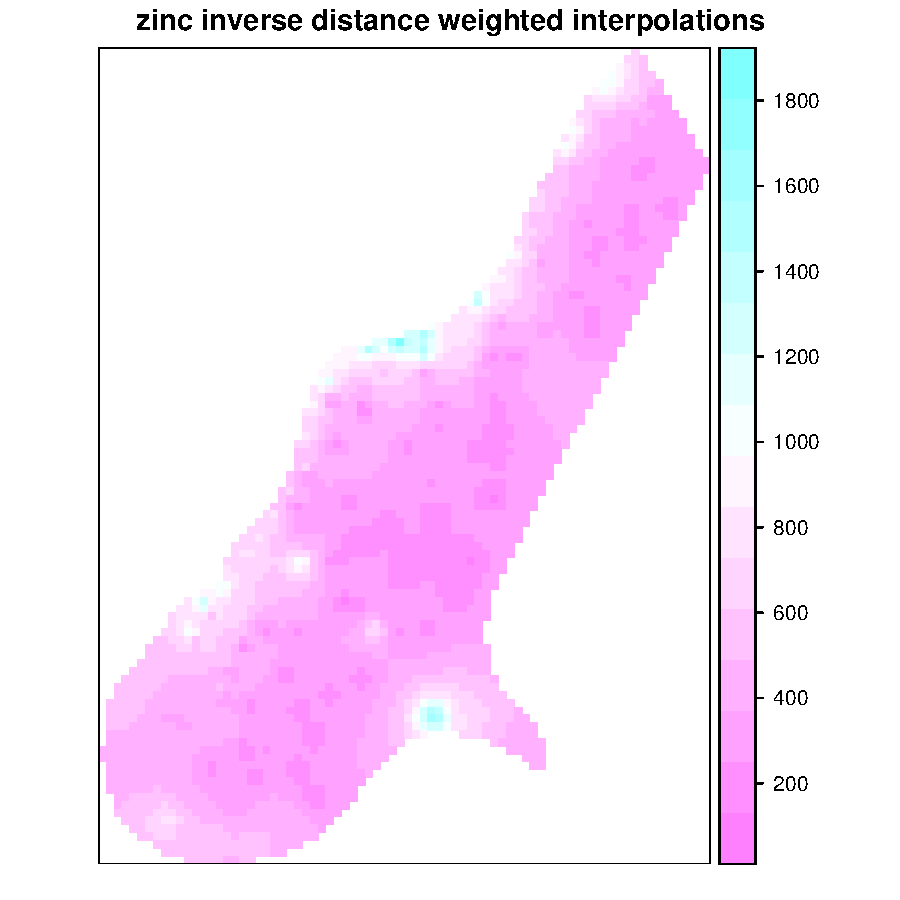
\includegraphics{gstat-004}

If you compare the bubble plot of zinc measurements with the map with
distances to the river, it becomes evident that the larger concentrations
are measured at locations close to the river. This relationship can be
linearized by log-transforming the zinc concentrations, and taking the
square root of distance to the river:

\begin{Schunk}
\begin{Sinput}
> plot(log(zinc) ~ sqrt(dist), meuse)
> abline(lm(log(zinc) ~ sqrt(dist), meuse))
\end{Sinput}
\end{Schunk}
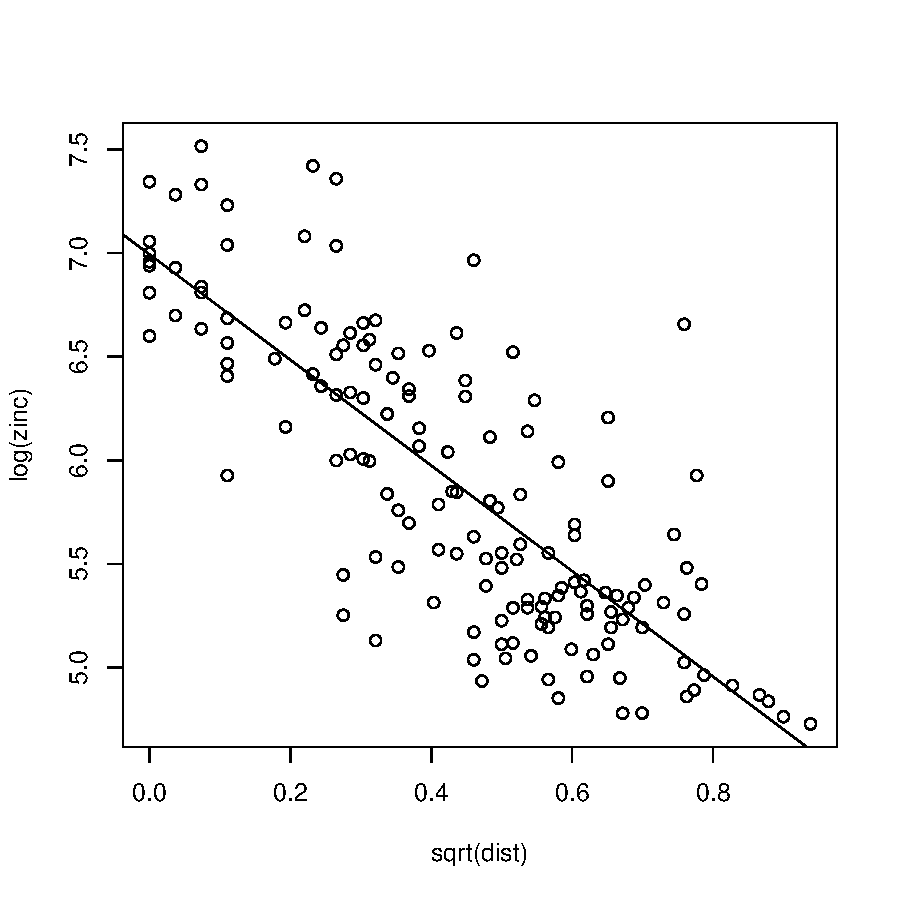
\includegraphics{gstat-005}

\section{Variograms }

Variograms are calculated using the function \code{variogram}, which
takes a formula as its first argument: \verb|log(zinc)~1| means that we
assume a constant trend for the variable log(zinc).

\begin{Schunk}
\begin{Sinput}
> lzn.vgm = variogram(log(zinc) ~ 1, meuse)
> lzn.vgm
\end{Sinput}
\begin{Soutput}
    np       dist     gamma dir.hor dir.ver   id
1   57   79.29244 0.1234479       0       0 var1
2  299  163.97367 0.2162185       0       0 var1
3  419  267.36483 0.3027859       0       0 var1
4  457  372.73542 0.4121448       0       0 var1
5  547  478.47670 0.4634128       0       0 var1
6  533  585.34058 0.5646933       0       0 var1
7  574  693.14526 0.5689683       0       0 var1
8  564  796.18365 0.6186769       0       0 var1
9  589  903.14650 0.6471479       0       0 var1
10 543 1011.29177 0.6915705       0       0 var1
11 500 1117.86235 0.7033984       0       0 var1
12 477 1221.32810 0.6038770       0       0 var1
13 452 1329.16407 0.6517158       0       0 var1
14 457 1437.25620 0.5665318       0       0 var1
15 415 1543.20248 0.5748227       0       0 var1
\end{Soutput}
\begin{Sinput}
> lzn.fit = fit.variogram(lzn.vgm, model = vgm(1, "Sph", 900, 1))
> lzn.fit
\end{Sinput}
\begin{Soutput}
  model      psill    range
1   Nug 0.05066243   0.0000
2   Sph 0.59060780 897.0209
\end{Soutput}
\begin{Sinput}
> plot(lzn.vgm, lzn.fit)
\end{Sinput}
\end{Schunk}

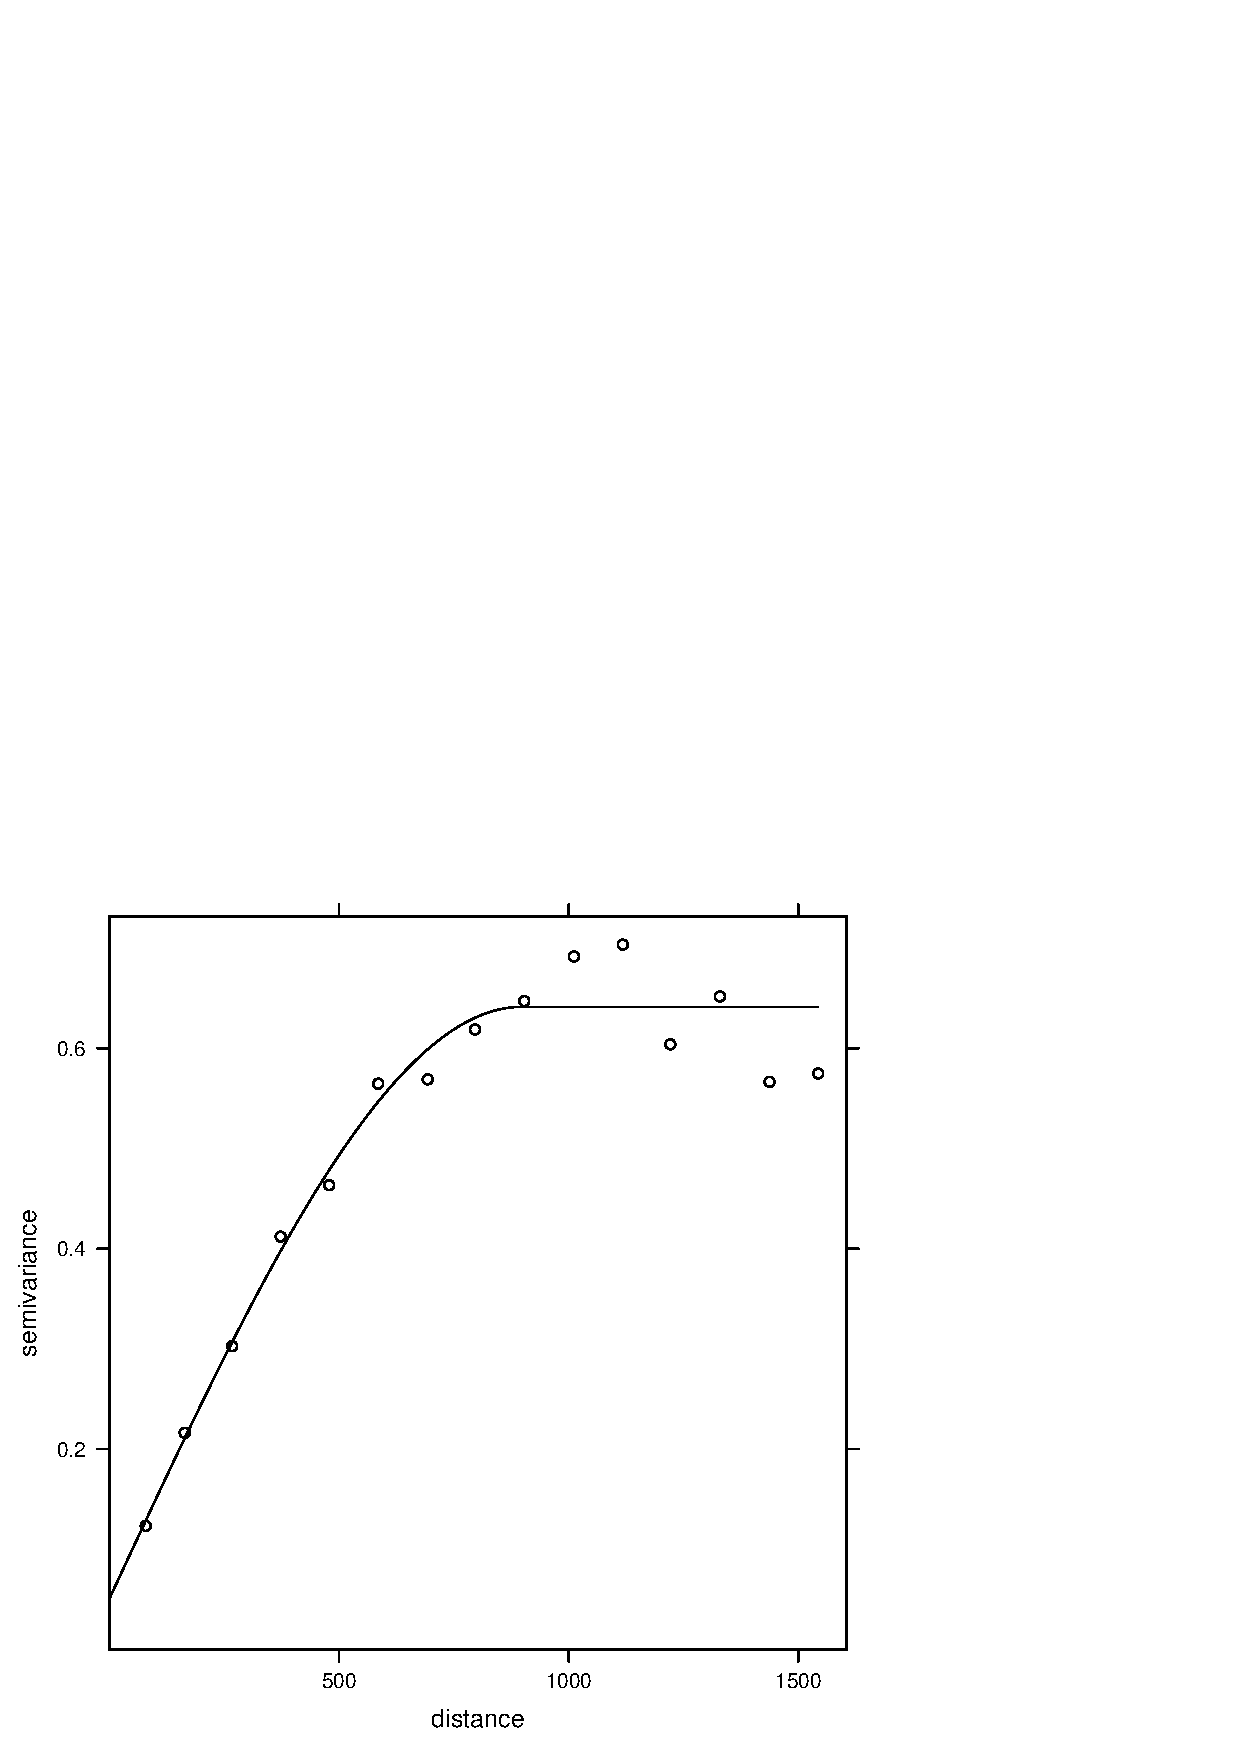
\includegraphics{gstat-007}

Instead of the constant mean, denoted by \verb|~1|, we can specify a
mean function, e.g. using \verb|~sqrt(dist)| as a predictor variable:

\begin{Schunk}
\begin{Sinput}
> lznr.vgm = variogram(log(zinc) ~ sqrt(dist), meuse)
> lznr.fit = fit.variogram(lznr.vgm, model = vgm(1, "Exp", 300, 
+     1))
> lznr.fit
\end{Sinput}
\begin{Soutput}
  model      psill    range
1   Nug 0.05712231   0.0000
2   Exp 0.17641559 340.3201
\end{Soutput}
\begin{Sinput}
> plot(lznr.vgm, lznr.fit)
\end{Sinput}
\end{Schunk}

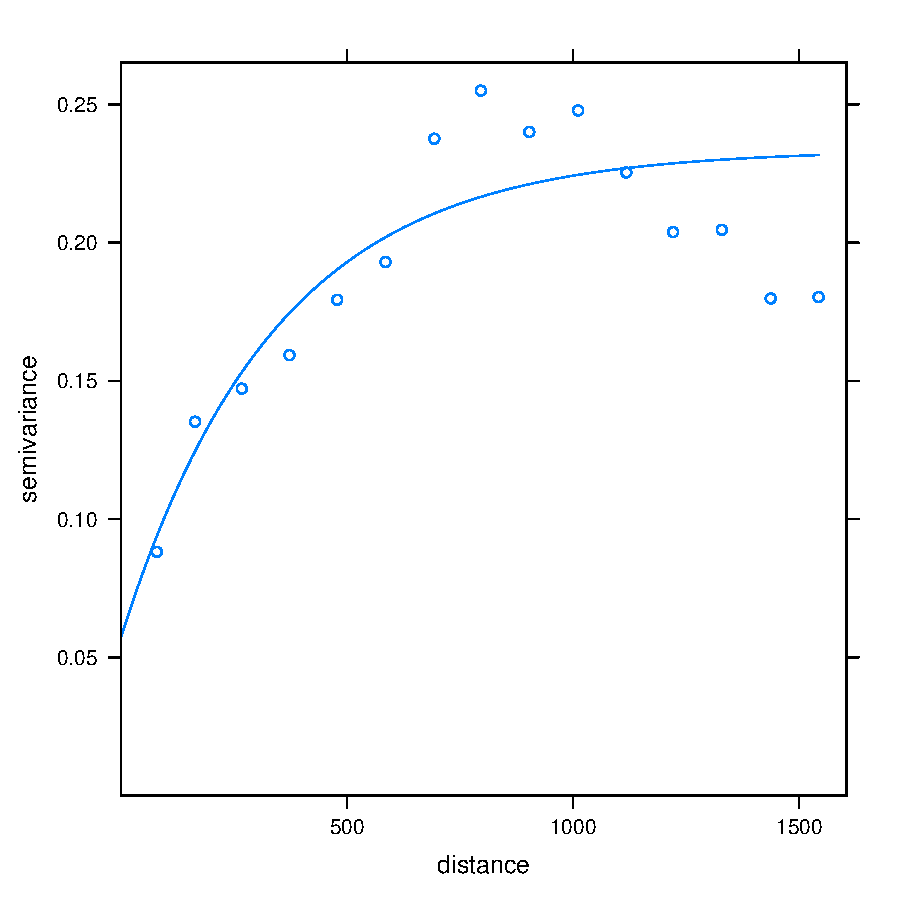
\includegraphics{gstat-009}

In this case, the variogram of residuals with respect to a fitted mean
function are shown. Residuals were calculated using ordinary least
squares.

\section{Kriging}

\begin{Schunk}
\begin{Sinput}
> lzn.kriged = krige(log(zinc) ~ 1, meuse, meuse.grid, model = lzn.fit)
\end{Sinput}
\begin{Soutput}
[using ordinary kriging]
\end{Soutput}
\begin{Sinput}
> spplot(lzn.kriged["var1.pred"])
\end{Sinput}
\end{Schunk}

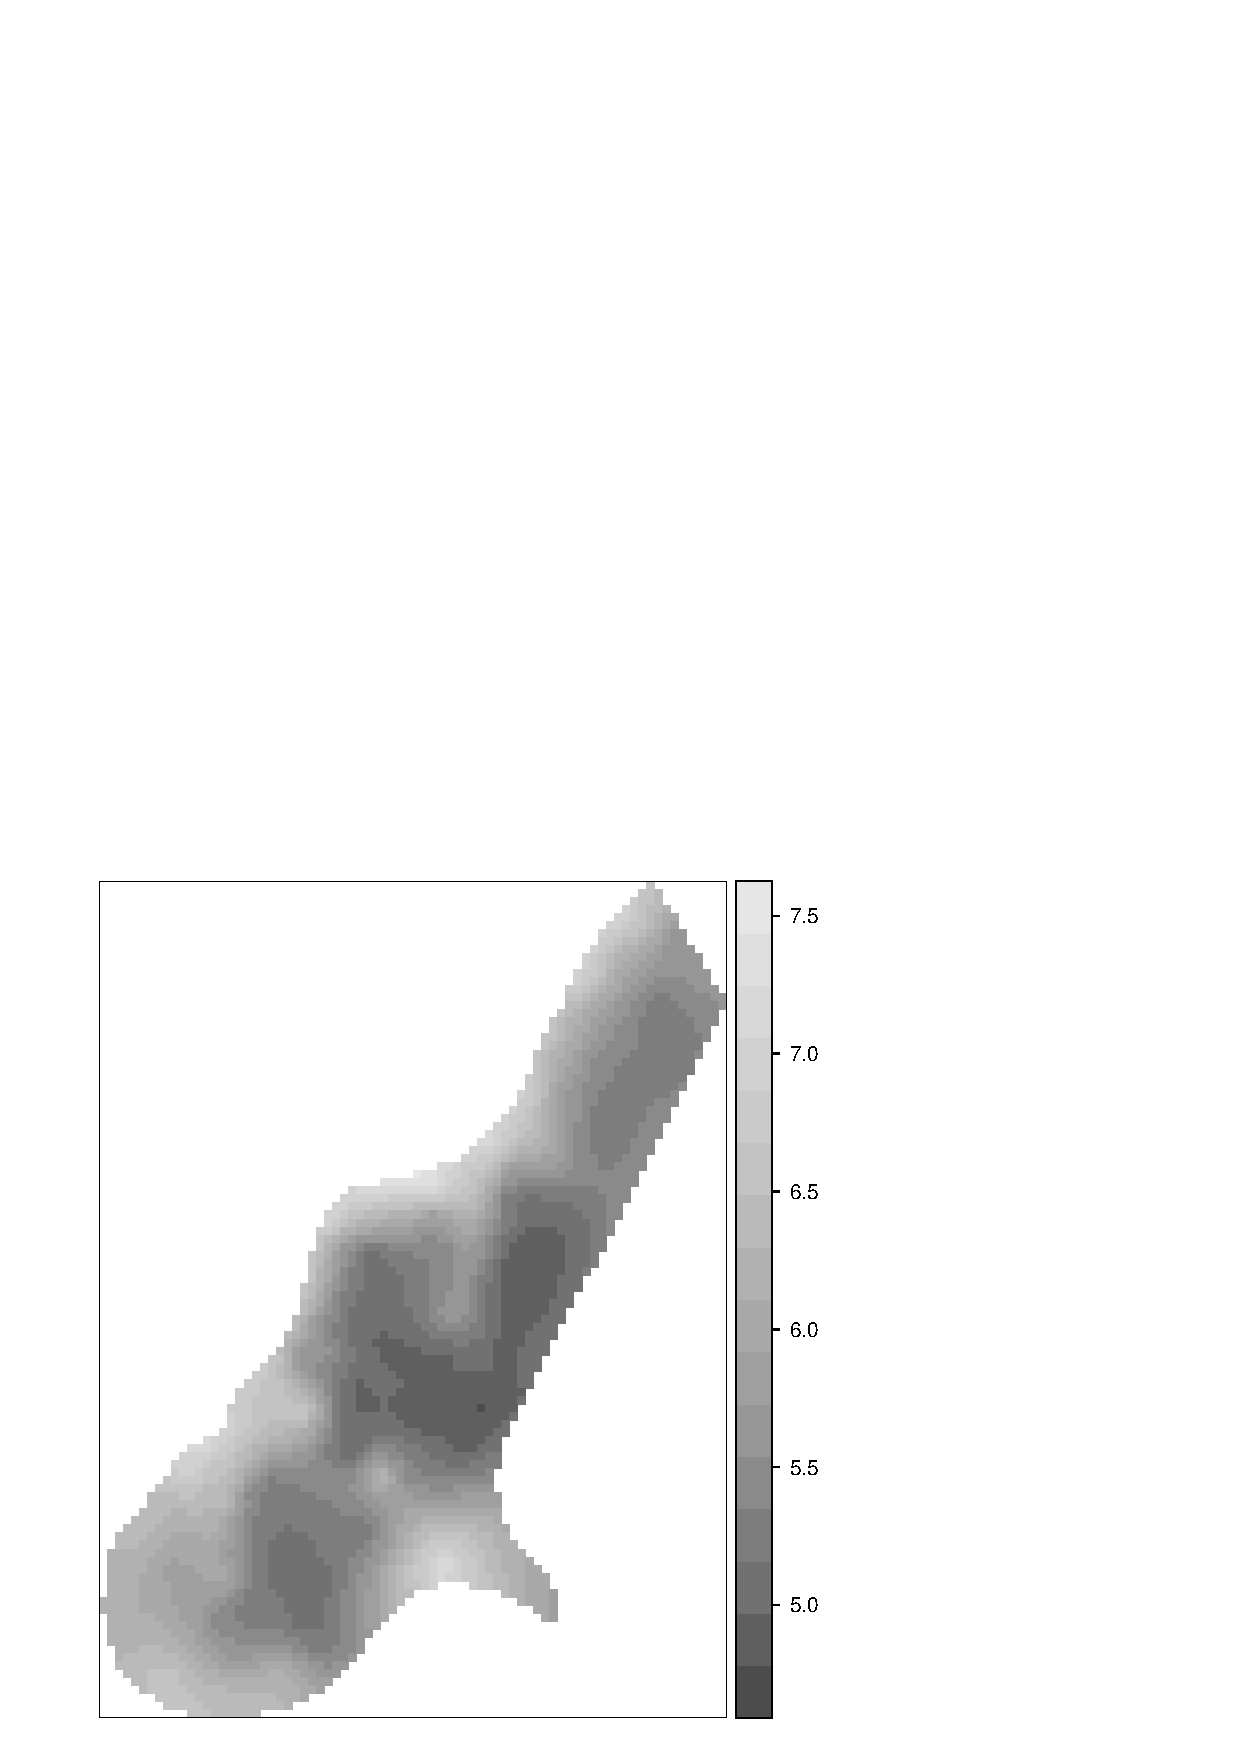
\includegraphics{gstat-011}

\section{Conditional simulation}
\begin{Schunk}
\begin{Sinput}
> lzn.condsim = krige(log(zinc) ~ 1, meuse, meuse.grid, model = lzn.fit, 
+     nmax = 30, nsim = 4)
\end{Sinput}
\begin{Soutput}
drawing 4 GLS realisations of beta...
[using conditional Gaussian simulation]
\end{Soutput}
\begin{Sinput}
> spplot(lzn.condsim, main = "three conditional simulations")
\end{Sinput}
\end{Schunk}

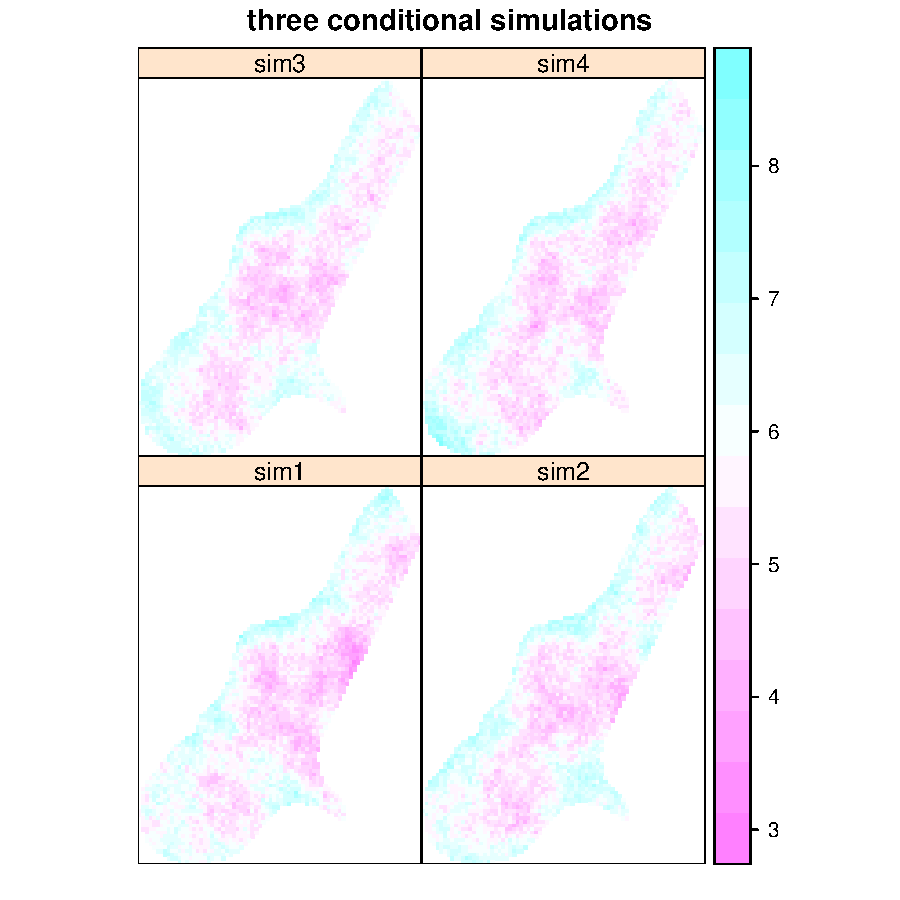
\includegraphics{gstat-013}

For UK/residuals:

\begin{Schunk}
\begin{Sinput}
> lzn.condsim2 = krige(log(zinc) ~ sqrt(dist), meuse, meuse.grid, 
+     model = lznr.fit, nmax = 30, nsim = 4)
\end{Sinput}
\begin{Soutput}
drawing 4 GLS realisations of beta...
[using conditional Gaussian simulation]
\end{Soutput}
\begin{Sinput}
> spplot(lzn.condsim2, main = "three UK conditional simulations")
\end{Sinput}
\end{Schunk}

\includegraphics{gstat-015}

\section{Directional variograms}
The following command calculates a directional sample variogram, where
directions are binned by direction angle alone. For two point pairs,
$Z(s)$ and $Z(s+h)$, the separation vector is $h$, and it has a direction.
Here, we will classify directions into four direction intervals:

\begin{Schunk}
\begin{Sinput}
> lzn.dir = variogram(log(zinc) ~ 1, meuse, alpha = c(0, 45, 90, 
+     135))
> lzndir.fit = vgm(0.59, "Sph", 1200, 0.05, anis = c(45, 0.4))
> plot(lzn.dir, lzndir.fit, as.table = TRUE)
\end{Sinput}
\end{Schunk}

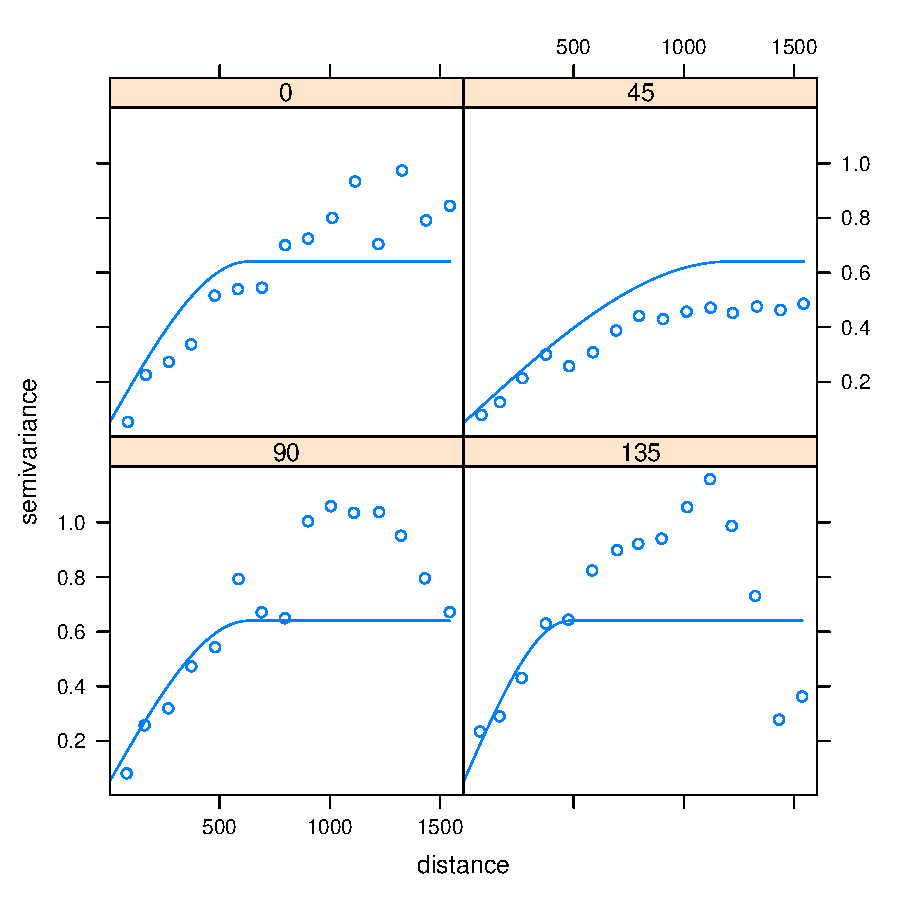
\includegraphics{gstat-017}

Looking at directions between 180 and 360 degrees will repeat the
image shown above, because the variogram is a symmetric measure:
$(Z(s)-Z(s+h))^2=(Z(s+h)-Z(s))^2$.

The first plot gives the variogram in the zero direction, which is
North; 90 degrees is East. By default, point pairs are assigned to the
directional variorgram panel with their nearest direction, so North
contains everything between -22.5 and 22.5 degrees (North-West to
North-East). After classifying by direction, point pairs are binned by
separation distance class, as is done in the usual omnidirectional case.

In the figure, the partial sill, nugget and model type of the model are
equal to those of the omnidirectional model fitted above; the range
is that in the direction with the largest range (45$^o$), and the
anisotropy ratio, the range in the 135 direction and the range in the
45 direction, estimated ``by eye'' by comparing the 45 and 135 degrees
sample variograms. Gstat does not fit anisotropy parameters automatically.

We do not claim that the model fitted here is ``best'' in some way; in
order to get to a better model we may want to look at more directions,
other directions (e.g. try {\tt alpha = c(22, 67, 112, 157) }), and to
variogram maps (see below). More elaborate approaches may use directions
in three dimentions, and want to furnter control the direction tolerance
(which may be set such that direction intervals overlap).

For the residual variogram from the linear regression model using
sqrt(dist) as covariate, the directional dependence is much less
obvious; the fitted model here is the fitted isotropic model (equal in
all directions).

\begin{Schunk}
\begin{Sinput}
> lznr.dir = variogram(log(zinc) ~ sqrt(dist), meuse, alpha = c(0, 
+     45, 90, 135))
> plot(lznr.dir, lznr.fit, as.table = TRUE)
\end{Sinput}
\end{Schunk}

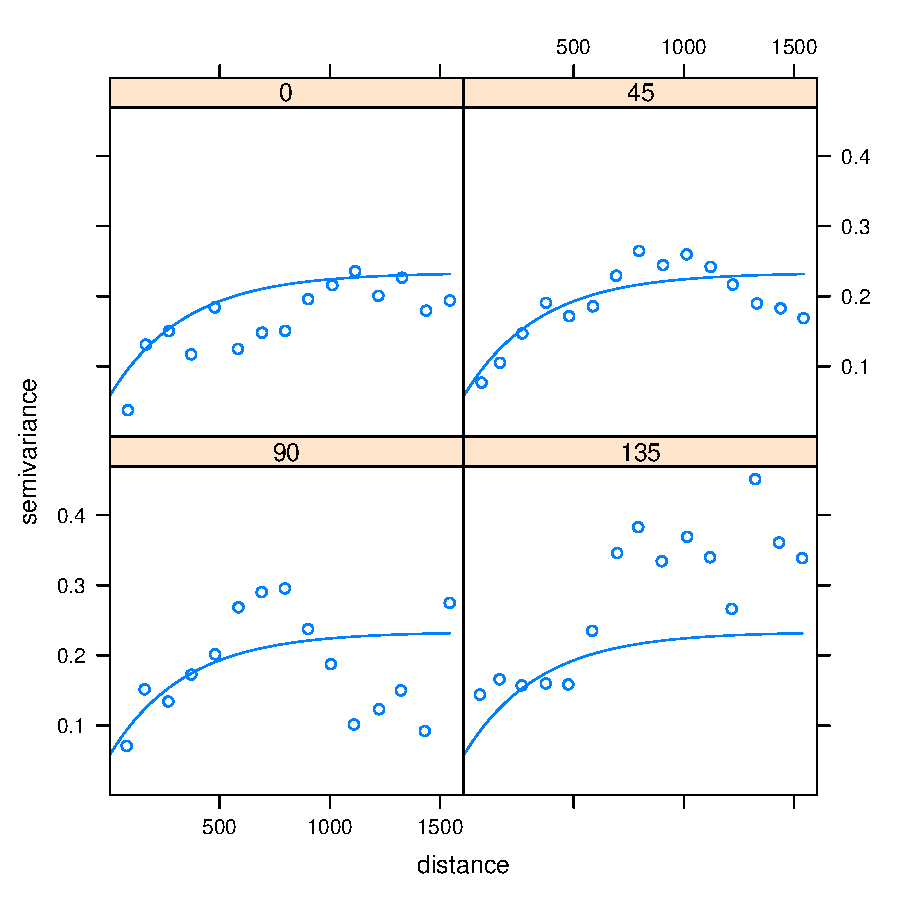
\includegraphics{gstat-019}

\section{Variogram maps}

Another means of looking at directional dependence in semivariograms
is obtained by looking at variogram maps. Instead of classifying
point pairs $Z(s)$ and $Z(s+h)$ by direction and distance class {\em
separately}, we can classify them {\em jointly}. If $h=\{x,y\}$ be the
two-dimentional coordinates of the separation vector, in the variogram
map the semivariance contribution of each point pair $(Z(s)-Z(s+h))^2$
is attributed to the grid cell in which $h$ lies. The map is centered
around $(0,0)$, as $h$ is geographical distance rather than geographical
location. Cutoff and width correspond to some extent to map extent
and cell size; the semivariance map is point symmetric around $(0,0)$,
as $\gamma(h)=\gamma(-h)$.

\begin{Schunk}
\begin{Sinput}
> vgm.map = variogram(log(zinc) ~ sqrt(dist), meuse, cutoff = 1500, 
+     width = 100, map = TRUE)
> plot(vgm.map, threshold = 5)
\end{Sinput}
\end{Schunk}

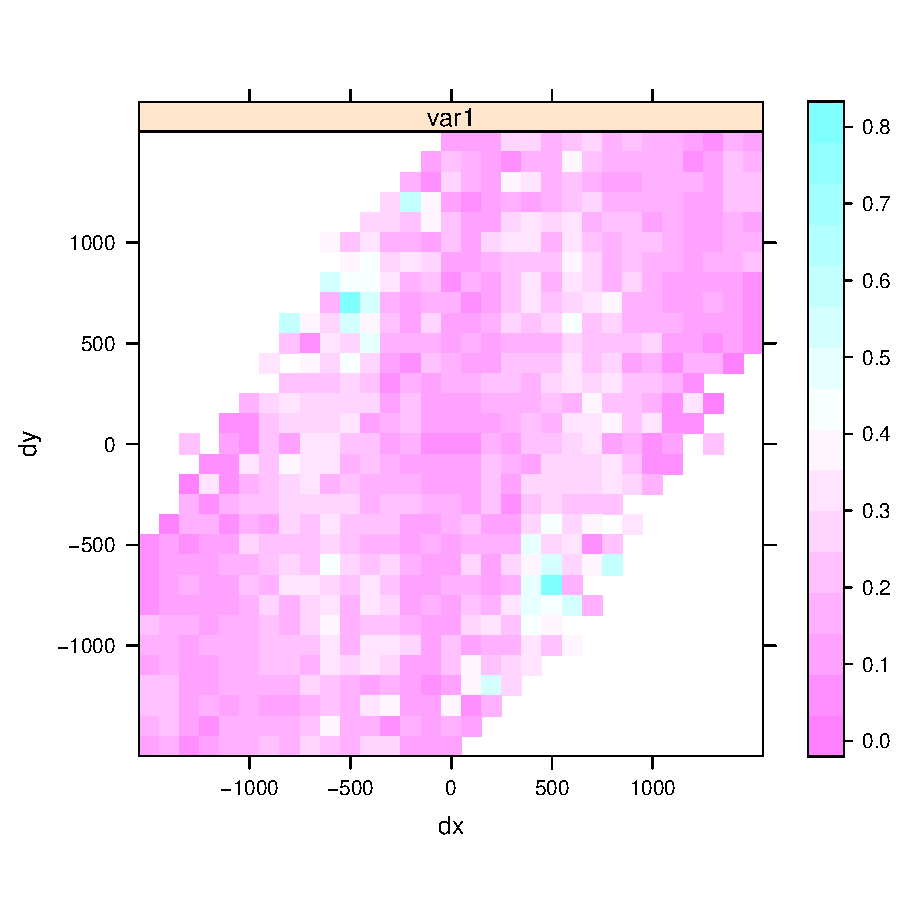
\includegraphics{gstat-021}

The threshold assures that only semivariogram map values based on at
least 5 point pairs are shown, removing too noisy estimation.

% The plot is plagued by one or two extreme values, corresponding to cells
% with very small number of point pairs, which should be removed.

\section{Cross variography}

Fitting a linear model of coregionalization.

\begin{Schunk}
\begin{Sinput}
> g = gstat(NULL, "log(zn)", log(zinc) ~ sqrt(dist), meuse)
> g = gstat(g, "log(cd)", log(cadmium) ~ sqrt(dist), meuse)
> g = gstat(g, "log(pb)", log(lead) ~ sqrt(dist), meuse)
> g = gstat(g, "log(cu)", log(copper) ~ sqrt(dist), meuse)
> v = variogram(g)
> g = gstat(g, model = vgm(1, "Exp", 300, 1), fill.all = TRUE)
> g.fit = fit.lmc(v, g)
> g.fit
\end{Sinput}
\begin{Soutput}
data:
log(zn) : formula = log(zinc)`~`sqrt(dist) ; data dim = 155 x 12
log(cd) : formula = log(cadmium)`~`sqrt(dist) ; data dim = 155 x 12
log(pb) : formula = log(lead)`~`sqrt(dist) ; data dim = 155 x 12
log(cu) : formula = log(copper)`~`sqrt(dist) ; data dim = 155 x 12
variograms:
                   model      psill range
log(zn)[1]           Nug 0.05141798     0
log(zn)[2]           Exp 0.17556219   300
log(cd)[1]           Nug 0.39996573     0
log(cd)[2]           Exp 0.47893816   300
log(pb)[1]           Nug 0.04770893     0
log(pb)[2]           Exp 0.21323027   300
log(cu)[1]           Nug 0.04577523     0
log(cu)[2]           Exp 0.07827374   300
log(zn).log(cd)[1]   Nug 0.09190848     0
log(zn).log(cd)[2]   Exp 0.24542024   300
log(zn).log(pb)[1]   Nug 0.04528367     0
log(zn).log(pb)[2]   Exp 0.18407011   300
log(cd).log(pb)[1]   Nug 0.06425412     0
log(cd).log(pb)[2]   Exp 0.25525359   300
log(zn).log(cu)[1]   Nug 0.02912806     0
log(zn).log(cu)[2]   Exp 0.10438748   300
log(cd).log(cu)[1]   Nug 0.09441635     0
log(cd).log(cu)[2]   Exp 0.13073936   300
log(pb).log(cu)[1]   Nug 0.02369778     0
log(pb).log(cu)[2]   Exp 0.10267516   300
\end{Soutput}
\begin{Sinput}
> plot(v, g.fit)
> vgm.map = variogram(g, cutoff = 1500, width = 100, map = TRUE)
> plot(vgm.map, threshold = 5, col.regions = bpy.colors(), xlab = "", 
+     ylab = "")
\end{Sinput}
\end{Schunk}

\includegraphics{gstat-023}

\includegraphics{gstat-024}

\section*{References}
\begin{itemize}
% \item Abrahamsen, P., F. Espen Benth, 2001. Kriging with inequality
% constraints.  Mathematical Geology 33 (6), 719--744.

% \item Bivand, R.S., 2003. Approaches to classes for spatial data in R.
% In: K.~Hornik \& F.~Leisch (Eds.), Proceedings of the 3rd International
% Workshop on Distributed Statistical Computing (DSC 2003) March 20--22,
% Vienna, Austria. ISSN 1609-395X; available from [1].

\item Diggle, P.J., J.A. Tawn, R.A. Moyeed, 1998. Model-based
geostatistics. Applied Statistics 47(3), pp 299-350.

% \item Pebesma, E.J., Wesseling, C.G., 1998. Gstat, a program for
% geostatistical modelling, prediction and simulation. Computers \&
% Geosciences, 24 (1), pp. 17--31.

\item Pebesma, E.J., 2004.  Multivariable geostatistics in S: the gstat
package.  Computers \& Geosciences \htmladdnormallink{30: 683-691}{%
http://www.sciencedirect.com/science/journal/00983004}.

% \item Ver Hoef, J.M., Cressie, N.A.C, 1993. Multivariable Spatial
% Prediction.  Mathematical Geology, 25 (2), pp. 219--240.

\item Wackernagel, H., 1998. Multivariate Geostatistics; an introduction
with applications, $2^{\mbox{nd}}$ edn., Springer, Berlin, 291 pp.

\end{itemize}

\end{document}

# g = gstat(NULL, "log.zinc", log(zinc)~1, meuse)
# g = gstat(g, "log.zinc.res", log(zinc)~sqrt(dist), meuse)
# lplot(vgm.map[["map"]], c("log.zinc", "log.zinc.res"))

% vim:syntax=tex
